\begin{surferPage}[30 Cuspides]{Uma Qu\'intica com 15 C\'uspides}
  Esta superf\'icie de grau $5$ (qu\'intica) tem $15$ singularidades do tipo $A_2$
    (chamadas c\'uspides); esta qu\'intica e uma s\'erie de superf\'icies relacionadas foram apresentadas num artigo por Oliver Labs em 2005.
    Cinco das c\'uspides parecem diferentes das outras dez.
    De facto, as cinco s\~ao singularidades $A_2^{++}$, e as outras $A_2^{+-}$ (ver a galeria das singularidades simples para mais informa\c c\~oes):

     \vspace*{-0.3em}
    \begin{center}
      \begin{tabular}{c@{\qquad}c}
        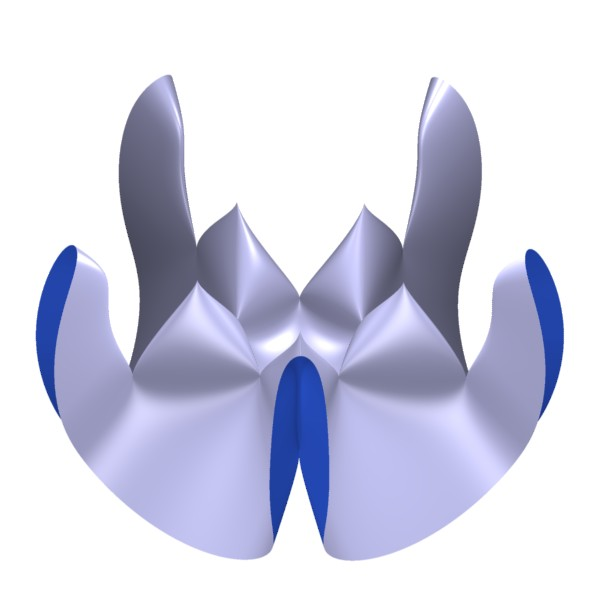
\includegraphics[height=1.2cm]{./../../common/images/dessins_quint_15a2}
        &
        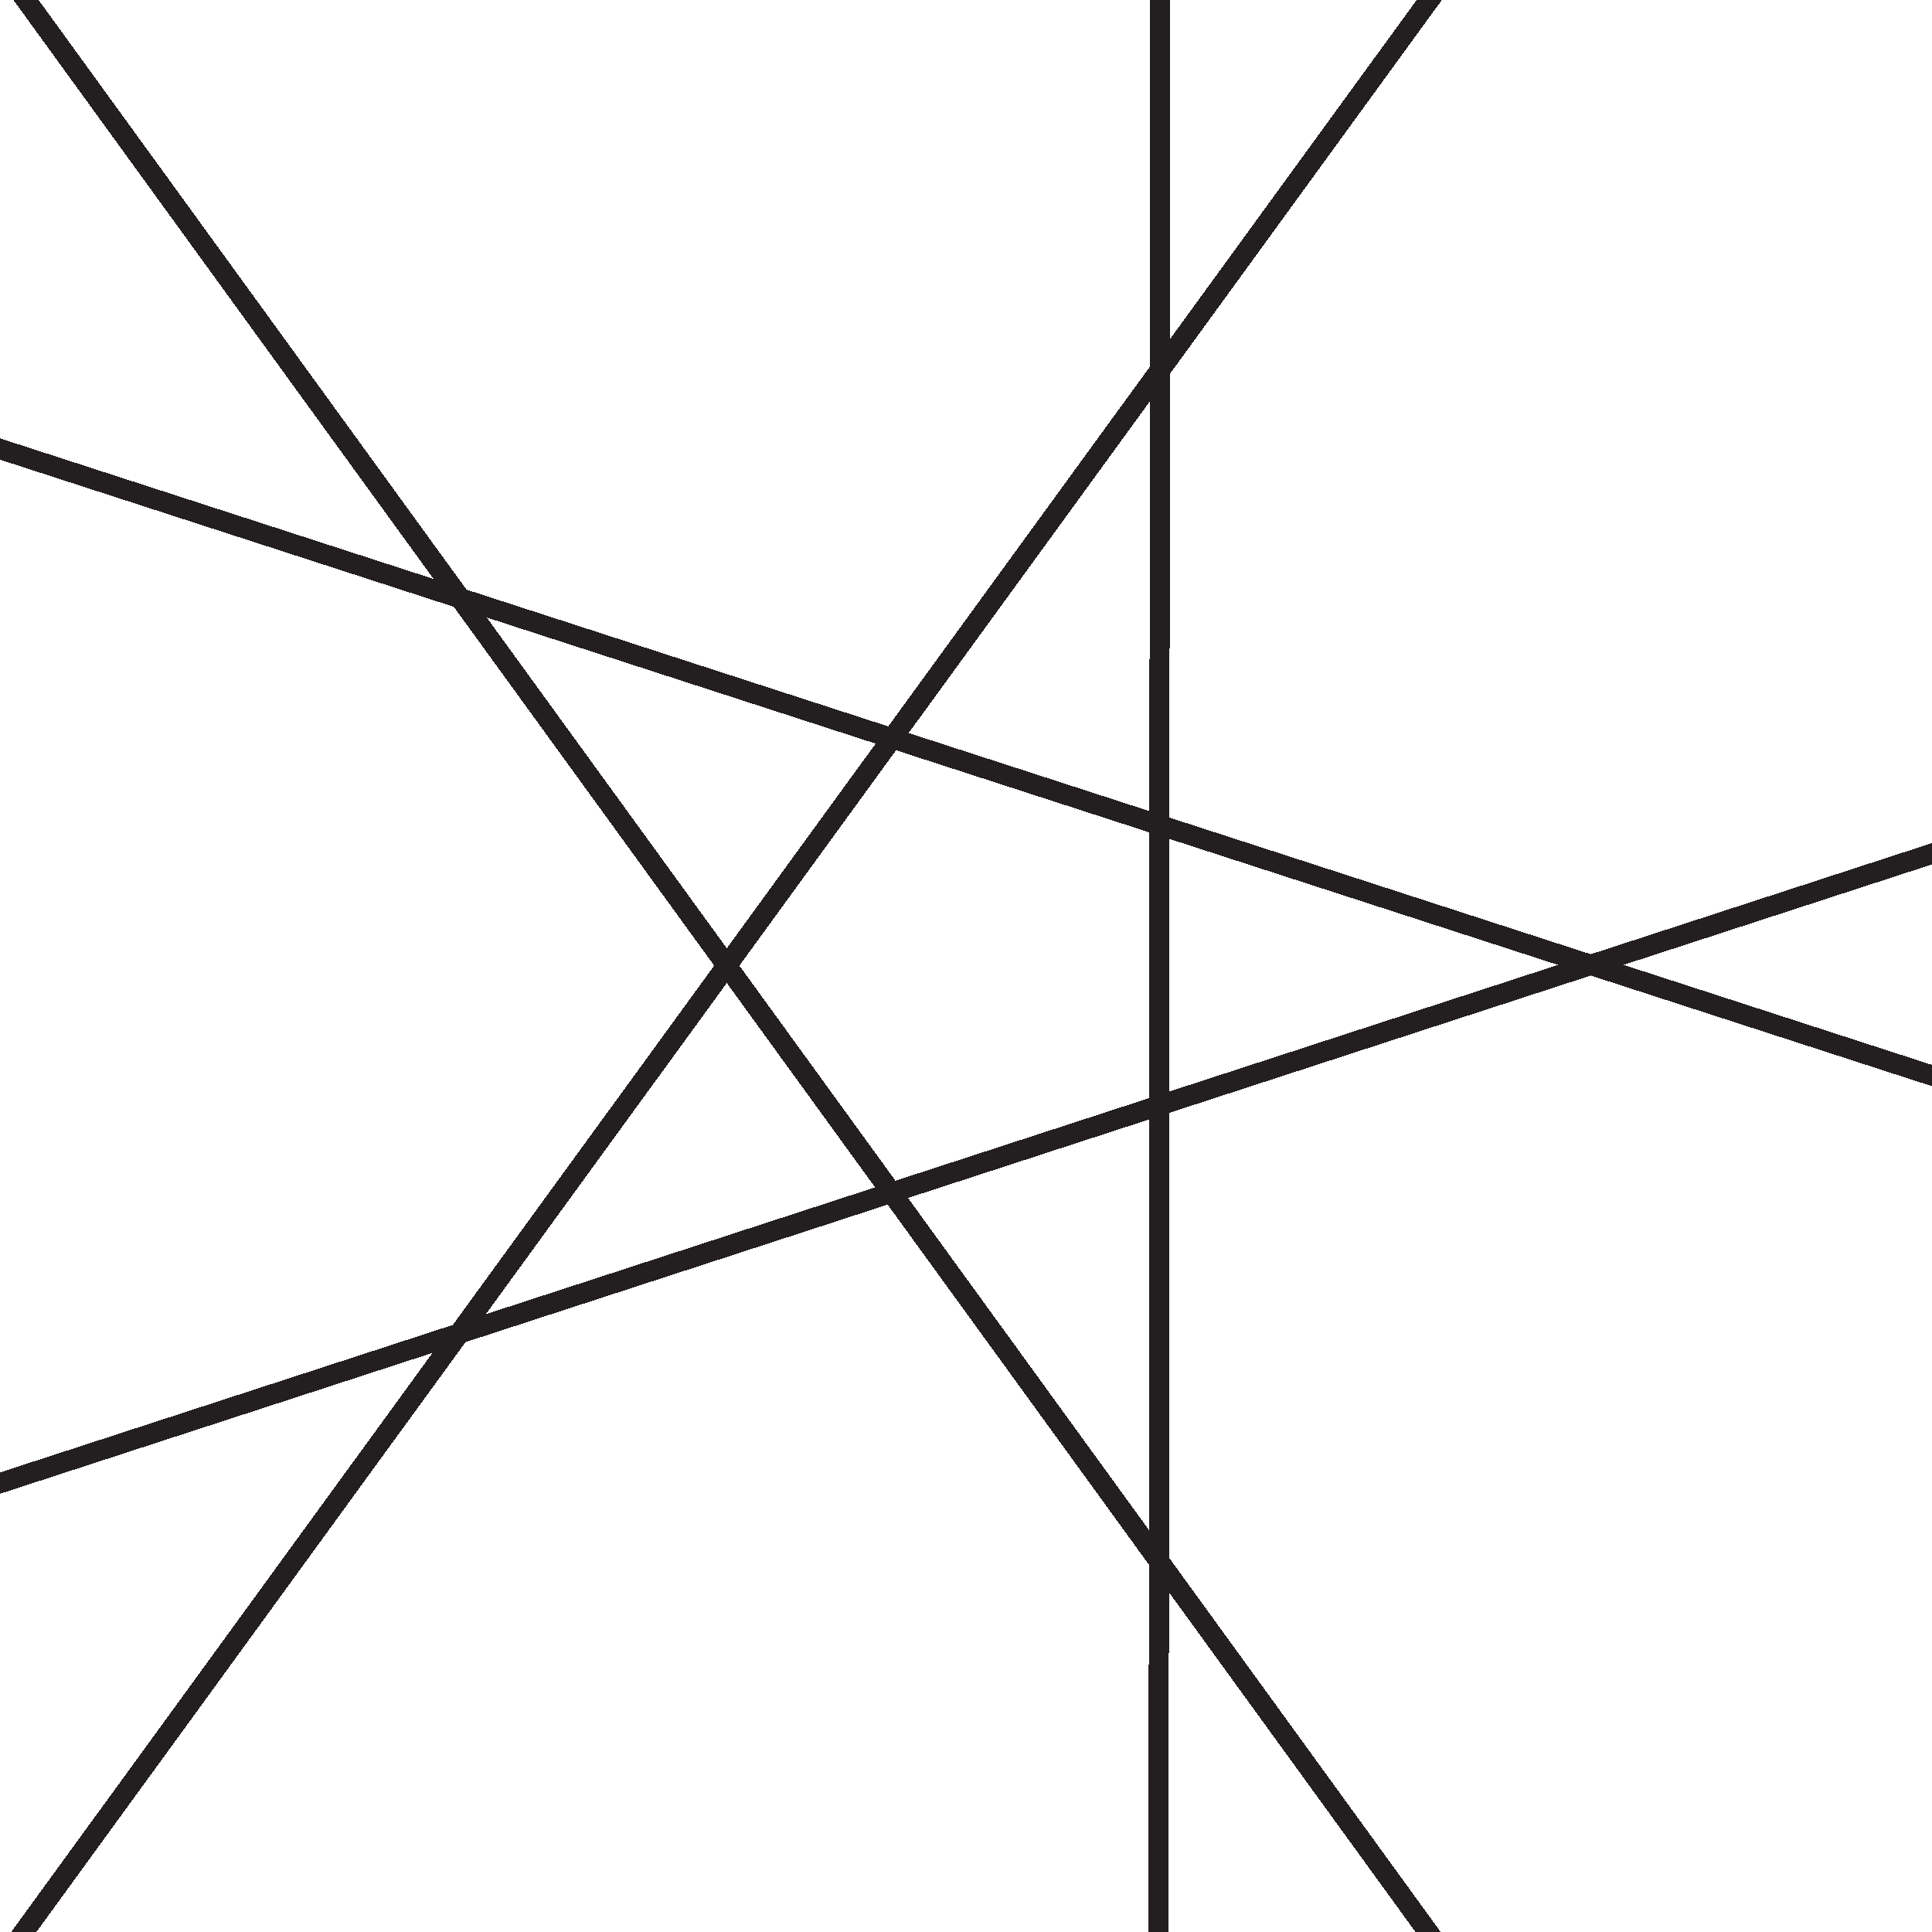
\includegraphics[height=1.2cm]{./../../common/images/rp5.pdf}
      \end{tabular}
    \end{center}
    \vspace*{-0.3em}    
    
    Esta superf\'icie tem uma equa\c c\~ao da forma
    $S_5(x,y) + t(z)=0,$
    onde $S_5(x,y)$ \'e um pent\'agono regular (imagem \`a direita) e $t(z)$ \'e uma variante dos polin\'omios de Tchebychev,  j\'a mencionados v\'arias vezes.

     Outra qu\'intica (\`a esquerda) com $15$ c\'uspides foi constru\'ida por Wolf Barth; ela est\'a relacionada com a C\'ubica de  Clebsch  (\`a direita) como se pode ver na imagem  do meio:

    \vspace*{-0.3em}
    \begin{center}
      \begin{tabular}{c@{\quad}c@{\quad}c}
        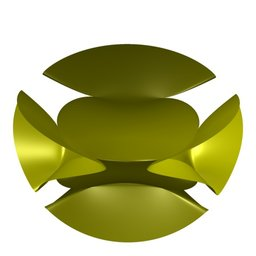
\includegraphics[height=1.2cm]{./../../common/images/barthquintic_green}
        &
        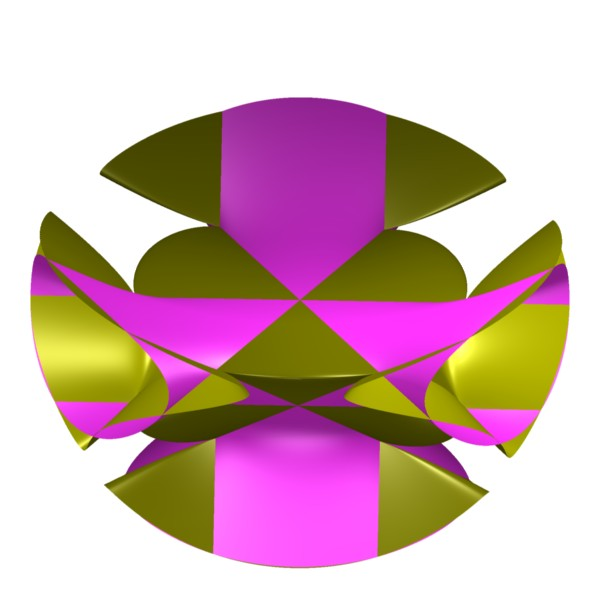
\includegraphics[height=1.2cm]{./../../common/images/barthquintic_clebschcubic}
        &
        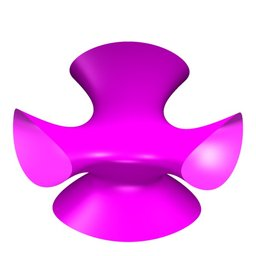
\includegraphics[height=1.2cm]{./../../common/images/clebschcubic_pink}
      \end{tabular}
    \end{center}
\end{surferPage}
